% ---------------------------------------------------------------------------
% Caderno 3 — Regressão e análise de variância
% Murilo Miguel Narciso, Instituto Militar de Engenharia.
% Compilação (MiKTeX fora do PATH):
%   $env:PATH = "C:\Users\Narcísius\AppData\Local\Programs\MiKTeX\miktex\bin\x64;" + $env:PATH
%   pdflatex -interaction=nonstopmode main.tex   (três vezes)
% ---------------------------------------------------------------------------
\documentclass{doeapostila}

% ---------------------------------------------------------------------------
% macros.tex — notação matemática comum aos cinco cadernos.
% Fixada antes de qualquer caderno começar, para os cinco não divergirem.
% Uso: % ---------------------------------------------------------------------------
% macros.tex — notação matemática comum aos cinco cadernos.
% Fixada antes de qualquer caderno começar, para os cinco não divergirem.
% Uso: % ---------------------------------------------------------------------------
% macros.tex — notação matemática comum aos cinco cadernos.
% Fixada antes de qualquer caderno começar, para os cinco não divergirem.
% Uso: \input{../estilo/macros} no preâmbulo de cada main.tex.
% ---------------------------------------------------------------------------

% Somas de quadrados
\newcommand{\SQT}{\mathrm{SQ}_{\mathrm{T}}}    % total
\newcommand{\SQR}{\mathrm{SQ}_{\mathrm{R}}}    % da regressão
\newcommand{\SQr}{\mathrm{SQ}_{\mathrm{r}}}    % residual
\newcommand{\SQfaj}{\mathrm{SQ}_{\mathrm{faj}}}% falta de ajuste
\newcommand{\SQep}{\mathrm{SQ}_{\mathrm{ep}}}  % erro puro

% Médias quadráticas: \MQ{R}, \MQ{r}, \MQ{faj}, \MQ{ep}
\newcommand{\MQ}[1]{\mathrm{MQ}_{\mathrm{#1}}}

% Coeficientes de determinação
\newcommand{\Rdois}{R^{2}}
\newcommand{\Rajus}{R^{2}_{\mathrm{aj}}}

% Efeitos: \efeito{1}, \efeito{12}
\newcommand{\efeito}[1]{E_{#1}}

% Álgebra matricial do ajuste por mínimos quadrados
\newcommand{\vetbeta}{\boldsymbol{\beta}}
\newcommand{\matX}{\mathbf{X}}
\newcommand{\vety}{\mathbf{y}}
 no preâmbulo de cada main.tex.
% ---------------------------------------------------------------------------

% Somas de quadrados
\newcommand{\SQT}{\mathrm{SQ}_{\mathrm{T}}}    % total
\newcommand{\SQR}{\mathrm{SQ}_{\mathrm{R}}}    % da regressão
\newcommand{\SQr}{\mathrm{SQ}_{\mathrm{r}}}    % residual
\newcommand{\SQfaj}{\mathrm{SQ}_{\mathrm{faj}}}% falta de ajuste
\newcommand{\SQep}{\mathrm{SQ}_{\mathrm{ep}}}  % erro puro

% Médias quadráticas: \MQ{R}, \MQ{r}, \MQ{faj}, \MQ{ep}
\newcommand{\MQ}[1]{\mathrm{MQ}_{\mathrm{#1}}}

% Coeficientes de determinação
\newcommand{\Rdois}{R^{2}}
\newcommand{\Rajus}{R^{2}_{\mathrm{aj}}}

% Efeitos: \efeito{1}, \efeito{12}
\newcommand{\efeito}[1]{E_{#1}}

% Álgebra matricial do ajuste por mínimos quadrados
\newcommand{\vetbeta}{\boldsymbol{\beta}}
\newcommand{\matX}{\mathbf{X}}
\newcommand{\vety}{\mathbf{y}}
 no preâmbulo de cada main.tex.
% ---------------------------------------------------------------------------

% Somas de quadrados
\newcommand{\SQT}{\mathrm{SQ}_{\mathrm{T}}}    % total
\newcommand{\SQR}{\mathrm{SQ}_{\mathrm{R}}}    % da regressão
\newcommand{\SQr}{\mathrm{SQ}_{\mathrm{r}}}    % residual
\newcommand{\SQfaj}{\mathrm{SQ}_{\mathrm{faj}}}% falta de ajuste
\newcommand{\SQep}{\mathrm{SQ}_{\mathrm{ep}}}  % erro puro

% Médias quadráticas: \MQ{R}, \MQ{r}, \MQ{faj}, \MQ{ep}
\newcommand{\MQ}[1]{\mathrm{MQ}_{\mathrm{#1}}}

% Coeficientes de determinação
\newcommand{\Rdois}{R^{2}}
\newcommand{\Rajus}{R^{2}_{\mathrm{aj}}}

% Efeitos: \efeito{1}, \efeito{12}
\newcommand{\efeito}[1]{E_{#1}}

% Álgebra matricial do ajuste por mínimos quadrados
\newcommand{\vetbeta}{\boldsymbol{\beta}}
\newcommand{\matX}{\mathbf{X}}
\newcommand{\vety}{\mathbf{y}}


% Vetor de erros aleatórios do modelo, na mesma convenção de \vetbeta,
% \matX e \vety definida em macros.tex. Não está no arquivo compartilhado
% porque só este caderno precisa distinguir o erro do modelo do resíduo
% observado; acrescentá-la aqui evita tocar em infraestrutura comum.
\newcommand{\vetepsilon}{\boldsymbol{\varepsilon}}

\definecaderno{3}{Regressão e análise de variância}

\graphicspath{{../figuras/out/}}

\begin{document}

\begin{center}
  {\large\bfseries Caderno 3\\Regressão e análise de variância}\par\smallskip
  {\normalsize Murilo Miguel Narciso}\par\smallskip
  {\footnotesize Instituto Militar de Engenharia \textbullet{} \today}
\end{center}

\vspace{0.6\baselineskip}

\noindent
Este caderno trata o planejamento fatorial do Caderno 2 como um problema de
regressão e, a partir dele, constrói o instrumental que permite julgar a
qualidade de um modelo ajustado: a decomposição da variância, o coeficiente
de determinação e sua versão ajustada, os testes de significância, o
valor-p, os diagnósticos de resíduo, a distinção entre falta de ajuste e
erro puro, e a validação por PRESS. Boa parte deste conteúdo não tem
tratamento direto no acervo de referência desta disciplina: o coeficiente de
determinação ajustado aparece em relatórios de software sem definição
alguma, o valor-p nunca é definido em português corrente, e a validação
cruzada um a um não é mencionada em nenhum documento consultado. Por isso
este é o caderno que fecha a maior lacuna do material didático original, e a
ênfase recai sobre esses pontos.

\vspace{0.6\baselineskip}

\tableofcontents

\section{Do efeito ao modelo}

No Caderno 2, a matriz de planejamento em variáveis codificadas serviu para
calcular efeitos por contraste: cada coluna de sinais $\pm 1$ definia uma
comparação de médias, e o produto $\matX^{\top}\vety$ produzia diretamente
as somas que, divididas pelo número de ensaios, geravam os efeitos e os
coeficientes. Essa mesma matriz $\matX$, entretanto, é também a matriz de
regressores de um modelo de regressão linear múltipla. Reconhecer essa
identidade é o que permite emprestar da regressão todo o instrumental de
inferência (testes de significância, intervalos de confiança, medidas de
qualidade de ajuste) para julgar planejamentos fatoriais, em vez de tratá-los
como um procedimento de cálculo isolado.

Considere-se o planejamento $2^{2}$ do catalisador, já apresentado no
Caderno 2 com os dados de \texttt{peixoto-2x2}. Em termos de médias por
célula, o vetor de respostas e a matriz de regressores, com a primeira
coluna reservada ao intercepto e a terceira à interação $x_{1}x_{2}$, são

\begin{equation}
  \vety = \begin{bmatrix} 59 \\ 90 \\ 54 \\ 68 \end{bmatrix},
  \qquad
  \matX = \begin{bmatrix}
    1 & -1 & -1 & +1 \\
    1 & +1 & -1 & -1 \\
    1 & -1 & +1 & -1 \\
    1 & +1 & +1 & +1
  \end{bmatrix} .
  \label{eq:matriz-2x2}
\end{equation}

Cada linha de $\matX$ é um ensaio; cada coluna, além da primeira, é o
contraste que define um efeito. A codificação em $\pm 1$ torna as colunas
ortogonais entre si, de modo que $\matX^{\top}\matX$ é uma matriz diagonal:
$4\,\mathbf{I}_4$ neste caso, com quatro ensaios. É essa propriedade,
estabelecida no Caderno 2 a partir da geometria do cubo, que faz cada
coeficiente de regressão poder ser calculado isoladamente dos demais, sem
que a inclusão ou a remoção de um termo altere a estimativa dos outros.
A Seção~\ref{sec:mmq} retoma esta mesma matriz para mostrar, com números,
como a fórmula geral de mínimos quadrados reproduz exatamente os efeitos
já conhecidos.

\section{O modelo linear nos parâmetros}

Um modelo é dito linear nos parâmetros quando a resposta é escrita como uma
combinação linear de coeficientes desconhecidos, multiplicando funções
conhecidas das variáveis de entrada. Em notação matricial,

\begin{equation}
  \vety = \matX\vetbeta + \vetepsilon ,
  \label{eq:modelo-geral}
\end{equation}

em que $\vety$ reúne as $n$ observações, $\matX$ é a matriz de
delineamento com $p$ colunas, $\vetbeta$ é o vetor de $p$ parâmetros
desconhecidos e $\vetepsilon$ é o vetor de erros aleatórios, não
observáveis, de média nula e variância $\sigma^{2}$ constante. A exigência
de linearidade recai sobre $\vetbeta$, não sobre as variáveis originais:
um modelo com termo quadrático, $y_i = \beta_0 + \beta_1 x_i + \beta_2
x_i^{2} + \varepsilon_i$, é linear nos parâmetros, porque $\beta_2$
multiplica a coluna conhecida $x_i^{2}$ da matriz $\matX$. O mesmo vale
para o modelo de potência que fecha este caderno, em que a linearização
por logaritmo transfere toda a não linearidade para dentro das colunas
conhecidas de $\matX$, deixando os parâmetros para serem estimados por um
ajuste inteiramente linear.

O vetor de respostas ajustadas é $\hat{\vety} = \matX\hat{\vetbeta}$, obtido
ao substituir o parâmetro verdadeiro, desconhecido, pela sua estimativa. A
diferença entre o modelo geral da Equação~\eqref{eq:modelo-geral} e sua
versão ajustada é o objeto da seção seguinte.

\section{Mínimos quadrados: a intuição antes da álgebra}
\label{sec:mmq}

Antes de qualquer manipulação matricial, vale fixar a imagem que sustenta o
método. A Figura~\ref{fig:nuvem-residuos} apresenta a nuvem de dezoito
observações de velocidade de queima de uma pólvora contra a pressão,
linearizadas por logaritmo (conjunto \texttt{peixoto-potencia}, detalhado
por completo na Seção~\ref{sec:aplicacao-final}), com a reta ajustada e os
resíduos desenhados como segmentos verticais entre cada ponto e a reta.

\begin{figure}[H]
  \centering
  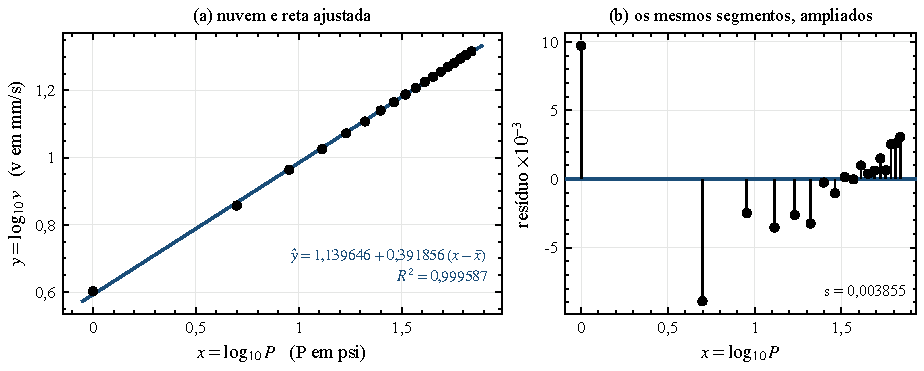
\includegraphics[width=\linewidth]{c3-nuvem-reta-residuos}
  \caption{À esquerda, a nuvem de pontos com a reta ajustada por mínimos
    quadrados. À direita, os mesmos segmentos residuais, ampliados em
    mil vezes para tornar visível a sua pequena magnitude diante do
    ajuste quase perfeito ($\Rdois = \num{0.999587}$). Dados de
    \texttt{peixoto-potencia}.}
  \label{fig:nuvem-residuos}
\end{figure}

O critério de mínimos quadrados escolhe, entre todas as retas possíveis,
aquela que minimiza a soma dos quadrados desses segmentos verticais, e não
a distância perpendicular à reta. A escolha da distância vertical não é
arbitrária: o objetivo do ajuste é prever $y$ a partir de $x$, de modo que
o erro relevante é o erro de previsão na escala da resposta, medido ao
longo do eixo que a reta pretende explicar. A escolha do quadrado, e não do
módulo da distância, garante uma solução única e diferenciável em toda
parte, e faz a soma minimizada coincidir exatamente com a soma de quadrados
residual que alimenta a análise de variância da Seção~\ref{sec:decomposicao}.

Antes de prosseguir, é necessário distinguir dois objetos que a notação
costuma confundir. O erro $\varepsilon_i$ da Equação~\eqref{eq:modelo-geral}
pertence ao modelo verdadeiro e desconhecido: é a distância entre a
observação e a reta que a natureza de fato obedece, e nunca é observado. O
resíduo $e_i = y_i - \hat{y}_i$, em contraste, é calculado a partir do
modelo ajustado, e depende de $\hat{\vetbeta}$, portanto da amostra
particular usada na estimação. O resíduo é a melhor estimativa disponível
do erro, mas não é o erro: duas amostras diferentes do mesmo processo
produzem o mesmo $\vetepsilon$ verdadeiro (no sentido distribucional) e
resíduos distintos, porque cada amostra estima $\vetbeta$ de forma
ligeiramente diferente.

A solução que minimiza $\sum_i e_i^{2} = (\vety - \matX\vetbeta)^{\top}
(\vety - \matX\vetbeta)$ em relação a $\vetbeta$ é obtida derivando essa
forma quadrática e igualando o gradiente a zero, o que conduz às equações
normais $\matX^{\top}\matX\vetbeta = \matX^{\top}\vety$. Sempre que
$\matX^{\top}\matX$ é inversível, a solução fecha-se em forma explícita:

\begin{equation}
  \hat{\vetbeta} = \left( \matX^{\top}\matX \right)^{-1} \matX^{\top}\vety .
  \label{eq:minimos-quadrados}
\end{equation}

\begin{aplicacao}{Mínimos quadrados no fatorial $2^{2}$}
  Com a matriz $\matX$ e o vetor $\vety$ da Equação~\eqref{eq:matriz-2x2},
  $\matX^{\top}\matX = 4\,\mathbf{I}_4$ em razão da ortogonalidade das
  colunas, de modo que $(\matX^{\top}\matX)^{-1} = \tfrac{1}{4}
  \mathbf{I}_4$. O vetor $\matX^{\top}\vety$ reúne a soma de todas as
  respostas na primeira posição e, nas demais, a soma de respostas com o
  sinal de cada coluna: $271$, $45$, $-27$ e $-17$. Aplicando a
  Equação~\eqref{eq:minimos-quadrados},
  \[
    \hat{\vetbeta} = \tfrac{1}{4}(271,\ 45,\ -27,\ -17)^{\top}
    = (67{,}75,\ 11{,}25,\ -6{,}75,\ -4{,}25)^{\top} ,
  \]
  reproduzindo exatamente a média global e os três coeficientes já obtidos
  no Caderno 2 pela via do contraste. A regressão e o contraste são, para
  este planejamento, o mesmo cálculo escrito de duas formas.
\end{aplicacao}

\section{Regressão linear simples}

No caso de um único regressor, é conveniente escrever o modelo na forma
centrada, $y_i = \beta_0 + \beta_1(x_i - \bar{x}) + \varepsilon_i$, com
$\bar{x}$ a média das observações de $x$. A centragem desloca a origem do
eixo para o centro da nuvem sem alterar a inclinação da reta, e traz duas
vantagens que justificam sua adoção como convenção. Em primeiro lugar, as
estimativas de mínimos quadrados assumem forma fechada simples,

\begin{equation}
  \hat{\beta}_0 = \bar{y} , \qquad
  \hat{\beta}_1 = \frac{\sum_i (x_i - \bar{x})\, y_i}
    {\sum_i (x_i - \bar{x})^{2}} .
  \label{eq:reg-simples}
\end{equation}

Em segundo lugar, a coluna do intercepto (uma coluna de uns) e a coluna do
regressor centrado tornam-se ortogonais, exatamente pela mesma razão que
tornava ortogonais as colunas do planejamento fatorial codificado: a soma
$\sum_i (x_i - \bar{x})$ é nula por construção. Disso decorre que
$\hat{\beta}_0$ e $\hat{\beta}_1$ são estatisticamente independentes, com
variâncias $\mathrm{Var}(\hat{\beta}_0) = \sigma^{2}/n$ e
$\mathrm{Var}(\hat{\beta}_1) = \sigma^{2} / \sum_i(x_i-\bar{x})^{2}$, sem
termo de covariância entre elas. É por essa razão que o modelo de potência
da Seção~\ref{sec:aplicacao-final} é escrito na forma $\hat{y} =
\hat{\beta}_0 + \hat{\beta}_1(x - \bar{x})$, com $\hat{\beta}_0 =
\num{1.139646}$ igual à média das dezoito respostas transformadas, tal como
indicado na Figura~\ref{fig:nuvem-residuos}.

\section{Decomposição da variância}
\label{sec:decomposicao}

A soma de quadrados total, que mede a variabilidade de toda a amostra em
torno da própria média, decompõe-se em uma parcela atribuível ao modelo e
uma parcela residual:

\begin{equation}
  \SQT = \sum_i (y_i - \bar{y})^{2} , \qquad
  \SQR = \sum_i (\hat{y}_i - \bar{y})^{2} , \qquad
  \SQr = \sum_i (y_i - \hat{y}_i)^{2} , \qquad
  \SQT = \SQR + \SQr .
  \label{eq:decomposicao-sq}
\end{equation}

A identidade da Equação~\eqref{eq:decomposicao-sq} é geométrica e não
depende da distribuição dos erros: decorre diretamente de $\hat{y}_i -
\bar{y}$ e $y_i - \hat{y}_i$ serem ortogonais entre si, consequência das
próprias equações normais que definiram $\hat{\vetbeta}$. Os graus de
liberdade seguem a mesma partição, com $n - 1$ para o total, $p - 1$ para a
regressão (o número de regressores além do intercepto) e $n - p$ para o
resíduo.

A Figura~\ref{fig:decomposicao} ilustra a decomposição sobre o conjunto
\texttt{peixoto-lin-quad}, dezoito observações de um mesmo experimento em
nove níveis de $x$ com duas réplicas cada, ajustado por uma reta.

\begin{figure}[H]
  \centering
  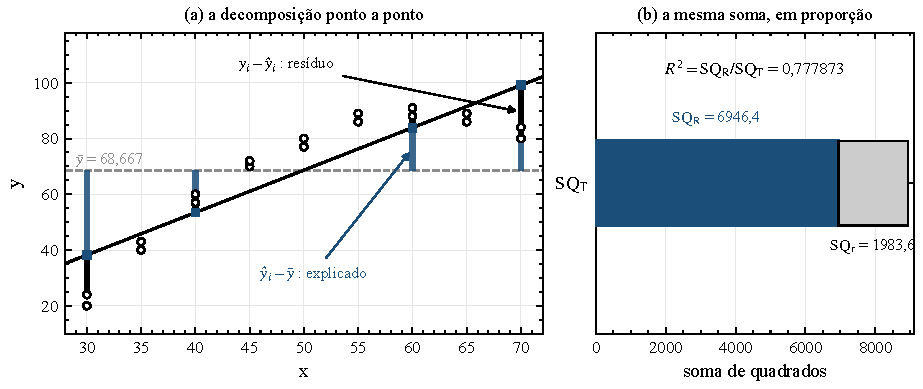
\includegraphics[width=\linewidth]{c3-decomposicao-sq}
  \caption{À esquerda, quatro observações escolhidas com a decomposição
    ponto a ponto entre a parcela explicada, $\hat{y}_i - \bar{y}$, e o
    resíduo, $y_i - \hat{y}_i$. À direita, a mesma soma de quadrados total
    representada em proporção, com $\SQR = \num{6946.4}$ e $\SQr =
    \num{1983.6}$ somando os $\SQT = \num{8930.0}$ do conjunto
    \texttt{peixoto-lin-quad}.}
  \label{fig:decomposicao}
\end{figure}

\section{O coeficiente de determinação}

O coeficiente de determinação é a fração da variabilidade total explicada
pelo modelo,

\begin{equation}
  \Rdois = \frac{\SQR}{\SQT} = 1 - \frac{\SQr}{\SQT} .
  \label{eq:r2}
\end{equation}

Por construção, $0 \leq \Rdois \leq 1$: o valor 1 corresponde a um ajuste
que reproduz exatamente todas as observações, e o valor 0, a um modelo que
não explica nada além da própria média. A leitura correta de $\Rdois$ é a
de proporção de variação explicada, não a de qualidade absoluta do modelo,
distinção retomada em detalhe na Seção~\ref{sec:teto-r2}.

\begin{aplicacao}{Análise de variância do modelo linear de \texttt{peixoto-lin-quad}}
  A Tabela~\ref{tab:anova-plq-linear} sintetiza a decomposição da variância
  da Figura~\ref{fig:decomposicao} na forma de uma tabela de análise de
  variância, com a média quadrática de cada fonte obtida ao dividir a soma
  de quadrados pelos respectivos graus de liberdade.

  \begin{table}[H]
    \centering
    \caption{Análise de variância do modelo linear ajustado a
      \texttt{peixoto-lin-quad}, $n = 18$.}
    \label{tab:anova-plq-linear}
    \begin{tabular}{l S[table-format=4.3] S[table-format=2.0] S[table-format=4.4]}
      \toprule
      {Fonte de variação} & {SQ} & {GL} & {MQ} \\
      \midrule
      Regressão & 6946.409  & 1  & 6946.409 \\
      Resíduo   & 1983.592  & 16 & 123.9745 \\
      \midrule
      Total     & 8930.000  & 17 & {} \\
      \bottomrule
    \end{tabular}
  \end{table}

  A razão entre as duas somas de quadrados fornece $\Rdois =
  \num{0.777873}$: cerca de 78\% da variação do conjunto é explicada pela
  reta ajustada. O restante, pouco mais de 22\%, permanece no resíduo, e a
  Seção~\ref{sec:falta-de-ajuste} mostra que essa parcela residual é quase
  inteiramente falta de ajuste, e não erro experimental.
\end{aplicacao}

\section{O coeficiente de determinação ajustado}
\label{sec:r2-ajustado}

O coeficiente de determinação carrega uma propriedade incômoda: ele nunca
diminui com a inclusão de um novo regressor no modelo, mesmo que esse termo
seja irrelevante para explicar a resposta. Isso ocorre porque mínimos
quadrados, ao acrescentar uma coluna a $\matX$, tem à sua disposição um
grau de liberdade a mais para reduzir a soma de quadrados residual, e o
mínimo de uma soma de quadrados nunca cresce quando o espaço de busca se
amplia. Em consequência, $\Rdois$ isoladamente não distingue um modelo que
melhorou de um modelo que apenas absorveu ruído.

O coeficiente de determinação ajustado corrige esse viés ao penalizar a
perda de graus de liberdade do resíduo:

\begin{equation}
  \Rajus = 1 - (1 - \Rdois) \cdot \frac{n-1}{n-p} ,
  \label{eq:r2-ajustado}
\end{equation}

em que $n$ é o número de observações e $p$ o número de parâmetros do
modelo, intercepto incluído. Diferentemente de $\Rdois$, $\Rajus$ pode
diminuir quando um termo é acrescentado: se a redução em $\SQr$ trazida
pelo novo regressor for pequena, o fator $(n-1)/(n-p)$ cresce mais depressa
do que $(1-\Rdois)$ diminui, e o produto aumenta, derrubando $\Rajus$. É
essa propriedade que torna $\Rajus$ útil para comparar modelos com número
diferente de termos, papel que $\Rdois$ sozinho não cumpre.

\begin{aplicacao}{Um modelo sem poder explicativo, e um que generaliza}
  A Tabela~\ref{tab:r2-ajustado} contrasta dois relatórios de software
  sobre planejamentos de dois fatores. O conjunto \texttt{origin-2x2}
  ajusta um modelo de efeitos principais a um fatorial $2^{2}$ com duas
  réplicas; o conjunto \texttt{aula-originpro} ajusta o mesmo tipo de
  modelo a outro fatorial $2^{2}$ com duas réplicas, resposta distinta.

  \begin{table}[H]
    \centering
    \caption{Coeficiente de determinação e sua versão ajustada em dois
      relatórios de software.}
    \label{tab:r2-ajustado}
    \begin{tabular}{l S[table-format=1.5] S[table-format=1.6]}
      \toprule
      {Conjunto} & {$\Rdois$} & {$\Rajus$} \\
      \midrule
      \texttt{origin-2x2}     & 0.34312  & 0.08037  \\
      \texttt{aula-originpro} & 0.866924 & 0.813693 \\
      \bottomrule
    \end{tabular}
  \end{table}

  No primeiro caso, o modelo explica apenas 34\% da variação observada, e o
  valor ajustado, 8\%, revela que quase todo esse poder explicativo
  aparente se deve ao número de parâmetros ajustados, não a uma relação
  real entre fatores e resposta. É um modelo sem poder explicativo prático,
  ainda que $\Rdois$ isoladamente não denunciasse isso com a mesma clareza.
  No segundo, $\Rdois$ e $\Rajus$ permanecem próximos um do outro,
  0{,}87 contra 0{,}81, o que indica que o poder explicativo do modelo não
  depende de forma crítica do número de parâmetros ajustados: é o padrão
  esperado de um modelo que de fato captura a relação entre fatores e
  resposta, e ao qual esta narrativa retorna nas
  Seções~\ref{sec:testes-significancia} e~\ref{sec:press}.
\end{aplicacao}

\section{O teto do coeficiente de determinação}
\label{sec:teto-r2}

Um conceito raramente discutido, e diretamente útil na prática, é o de que
$\Rdois$ tem um teto imposto pelo próprio ruído experimental, teto que
nenhum modelo, por melhor que seja, consegue ultrapassar. Quando existem
réplicas genuínas, a soma de quadrados residual nunca pode ficar abaixo da
soma de quadrados de erro puro $\SQep$, definida no
Caderno 1 e retomada na Seção~\ref{sec:falta-de-ajuste} como a
variabilidade interna aos pontos replicados, que nenhuma forma funcional
consegue reduzir por depender apenas da dispersão entre réplicas. Segue que
a fração máxima de variação explicável por qualquer modelo, por mais
flexível que seja, é

\begin{equation}
  \Rdois_{\max} = \frac{\SQT - \SQep}{\SQT} .
  \label{eq:teto-r2}
\end{equation}

Exigir de um modelo um $\Rdois$ acima desse teto é exigir o impossível: é
pedir que o ajuste explique inclusive a variação que é, por definição,
ruído puro, sem relação alguma com os fatores controlados. Ensaios com
grande variabilidade de medição têm teto baixo, e nenhuma sofisticação de
modelo compensa essa limitação; ensaios muito controlados, como o de
laboratório de calibração, têm teto próximo de 1, e um $\Rdois$
modesto nesse contexto já é sinal de modelo inadequado.

\begin{aplicacao}{O teto de \texttt{peixoto-lin-quad}}
  Para o conjunto \texttt{peixoto-lin-quad}, com $\SQT = \num{8930}$ e
  $\SQep = \num{45}$ obtidos das duas réplicas em cada um dos nove níveis
  de $x$, o teto vale
  \[
    \Rdois_{\max} = \frac{8930 - 45}{8930} = \num{0.994961} ,
  \]
  isto é, cerca de 99{,}5\%. O modelo quadrático da
  Seção~\ref{sec:falta-de-ajuste}, com $\Rdois = \num{0.993461}$, aproxima-se
  desse teto de perto, o que confirma que praticamente toda a variação
  explicável já foi capturada e que pouco resta a ganhar ao complicar ainda
  mais o modelo.
\end{aplicacao}

\section{Testes de significância}
\label{sec:testes-significancia}

Duas perguntas distintas precisam de testes distintos. A primeira, se o
modelo como um todo explica uma fração de variação maior do que se
explicaria por acaso, responde-se pelo teste $F$ da regressão,

\begin{equation}
  F = \frac{\MQ{R}}{\MQ{r}} = \frac{\SQR/(p-1)}{\SQr/(n-p)} ,
  \label{eq:teste-f}
\end{equation}

comparado ao quantil $F_{\alpha}(p-1,\,n-p)$ sob a hipótese nula de que
todos os coeficientes, exceto o intercepto, são nulos. A segunda pergunta,
se um coeficiente específico é diferente de zero, responde-se pelo teste
$t$ individual, $t = \hat{\beta}_j / \mathrm{EP}(\hat{\beta}_j)$, com
$n-p$ graus de liberdade. Quando o termo testado tem um único grau de
liberdade, como um efeito principal em um planejamento fatorial, as duas
perguntas coincidem, e $t^{2} = F$: o teste $t$ do coeficiente e o teste
$F$ daquele termo isolado na tabela de análise de variância são a mesma
comparação escrita de duas formas.

\begin{aplicacao}{Um termo relevante, um termo irrelevante}
  A Tabela~\ref{tab:testes-coef} retoma os dois conjuntos da
  Seção~\ref{sec:r2-ajustado} e reporta o teste $t$ de cada coeficiente ao
  lado do teste $F$ equivalente daquele termo na análise de variância,
  confirmando a identidade $t^{2} = F$ em cada linha.

  \begin{table}[H]
    \centering
    \caption{Testes de significância dos efeitos principais em
      \texttt{origin-2x2} (5 graus de liberdade do erro) e em
      \texttt{aula-originpro} (5 graus de liberdade do erro).}
    \label{tab:testes-coef}
    \begin{tabular}{l l S[table-format=-2.5] S[table-format=2.5] S[table-format=1.5]}
      \toprule
      {Conjunto} & {Termo} & {$t$} & {$F$} & {$p$} \\
      \midrule
      \texttt{origin-2x2}     & Fibra   & 0.38139  & 0.14546  & 0.71858 \\
      \texttt{origin-2x2}     & Cimento & -1.57044 & 2.46628  & 0.17711 \\
      \texttt{aula-originpro} & cond    & 2.93520  & 8.61538  & 0.03244 \\
      \texttt{aula-originpro} & par     & 4.89460  & 23.95706 & 0.00450 \\
      \bottomrule
    \end{tabular}
  \end{table}

  Em \texttt{origin-2x2}, nenhum dos dois efeitos principais se distingue
  do ruído a 5\%: os valores-$p$, 0{,}72 e 0{,}18, estão muito acima do
  limiar convencional. Em \texttt{aula-originpro}, os dois efeitos são
  significativos, com valores-$p$ de 0{,}032 e 0{,}0045. É o mesmo par de
  fatores, condição e pressão de compactação, medido em resposta
  diferente, com conclusões opostas quanto à significância. Vale ainda
  registrar, como referência de grandeza, que o ajuste de
  \texttt{peixoto-potencia} da Seção~\ref{sec:aplicacao-final} produz
  $F = \num{38739.5}$ para o coeficiente angular, uma ordem de grandeza
  típica de um ajuste quase determinístico, muito distante da fronteira de
  significância que separa os dois conjuntos desta tabela.
\end{aplicacao}

\section{O valor-p}
\label{sec:valor-p}

O valor-$p$ é a probabilidade de observar, sob a hipótese nula, uma
estatística de teste tão extrema ou mais extrema do que a que foi de fato
calculada a partir dos dados. Para o teste $t$ de um coeficiente, é a
probabilidade de uma variável $t$ com $n-p$ graus de liberdade exceder, em
módulo, o valor observado. Quanto menor o valor-$p$, menos compatíveis os
dados são com a hipótese de que o coeficiente vale zero, e maior a
evidência a favor de que o efeito é real.

É igualmente importante fixar o que o valor-$p$ não significa. Ele não é a
probabilidade de a hipótese nula ser verdadeira, nem a probabilidade de o
efeito estimado ser real, nem uma medida do tamanho ou da relevância
prática do efeito. Um efeito pequeno e sem importância pode ter valor-$p$
minúsculo se a amostra for grande o bastante, e um efeito grande pode ter
valor-$p$ elevado se a variabilidade do erro experimental for grande ou o
número de graus de liberdade, pequeno, como ocorre nos cinco graus de
liberdade de \texttt{origin-2x2} da Tabela~\ref{tab:testes-coef}: os
efeitos de fibra e cimento podem ser reais e ainda assim não se
distinguirem do ruído nessa amostra particular.

O limiar de 5\%, tão citado na prática, é convenção adotada por Ronald
Fisher no início do século XX, e não uma lei da natureza. Nada na
matemática do teste distingue 0{,}049 de 0{,}051; a diferença de conclusão
entre os dois valores é um artefato de onde a convenção traçou a linha, não
uma mudança substantiva na evidência. Áreas de decisão que exigem mais
cautela, como ensaios clínicos, costumam adotar limiares mais rigorosos; a
engenharia de materiais, em contrapartida, frequentemente aceita 10\% em
etapas de triagem, quando o custo de descartar por engano um fator
relevante supera o custo de investigar um fator que depois se revela
irrelevante. A escolha do limiar deveria refletir esse balanço de custos, e
não ser copiada de um relatório de software sem reflexão.

\section{Intervalos de confiança dos coeficientes e da resposta prevista}

Cada coeficiente estimado tem um intervalo de confiança da forma
$\hat{\beta}_j \pm t_{\alpha/2,\,n-p}\cdot \mathrm{EP}(\hat{\beta}_j)$, com
o mesmo quantil $t$ que alimenta o teste da Seção~\ref{sec:testes-significancia}.
Para a resposta prevista em um ponto $x_0$, o intervalo se apoia na
variância da previsão,

\begin{equation}
  \mathrm{Var}(\hat{y}_0) = \MQ{r}
  \left[ \frac{1}{n} + \frac{(x_0 - \bar{x})^{2}}
  {\sum_i (x_i - \bar{x})^{2}} \right] ,
  \label{eq:var-previsao}
\end{equation}

que cresce à medida que $x_0$ se afasta do centro $\bar{x}$ da faixa
experimental, por causa do segundo termo entre colchetes. O resultado
prático é uma banda de confiança em forma de ampulheta em torno da reta
ajustada, estreita perto do centro dos dados e alargando-se nas
extremidades. Extrapolar a previsão para além da faixa efetivamente
observada amplia essa incerteza sem limite, e a Equação~\eqref{eq:var-previsao}
não é válida fora da região onde os dados foram coletados, porque nada
garante que a forma funcional ajustada continue apropriada além dela.

\begin{aplicacao}{Precisão dos coeficientes em \texttt{peixoto-potencia}}
  Com dezoito pontos e $n - p = 16$ graus de liberdade, o quantil $t$ a
  95\% vale $\num{2.119905}$. Os intervalos de confiança resultantes para
  os dois coeficientes do modelo centrado são
  \[
    \hat{\beta}_0 = \num{1.139646} \pm \num{0.001926} , \qquad
    \hat{\beta}_1 = \num{0.391856} \pm \num{0.004221} ,
  \]
  ambos com semi-amplitude bem menor que 1\% do valor estimado, reflexo
  direto do ajuste quase perfeito já anunciado pelo $\Rdois = \num{0.999587}$
  da Figura~\ref{fig:nuvem-residuos}. A pequena magnitude do resíduo,
  visível apenas quando ampliada em mil vezes no painel (b) daquela
  figura, é a mesma causa que torna aqui os coeficientes tão precisamente
  determinados.
\end{aplicacao}

\section{Resíduos e normalidade}

A validade dos testes $t$ e $F$ apoia-se em hipóteses sobre o erro
$\varepsilon_i$: média nula, variância constante e distribuição próxima da
normal. Como o erro verdadeiro não é observável, essas hipóteses são
verificadas por meio do resíduo, sua melhor aproximação disponível, com
quatro gráficos de diagnóstico de uso corrente.

\begin{figure}[H]
  \centering
  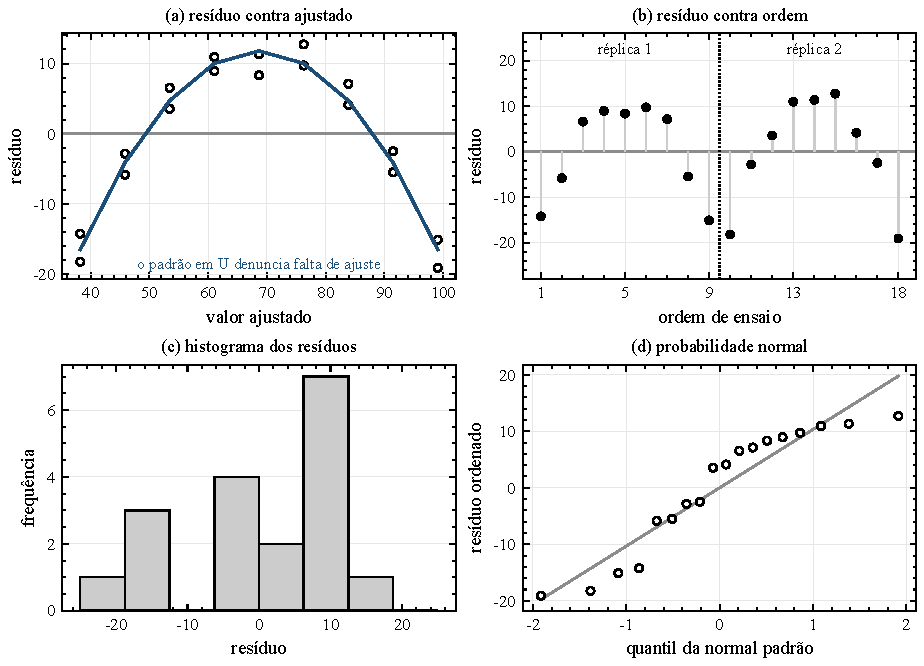
\includegraphics[width=\linewidth]{c3-diagnosticos-residuo}
  \caption{Quatro diagnósticos de resíduo para o modelo linear ajustado a
    \texttt{peixoto-lin-quad}. (a) resíduo contra valor ajustado, com um
    padrão em curva que denuncia falta de ajuste; (b) resíduo contra a
    ordem de execução, separado por réplica, sem tendência aparente;
    (c) histograma dos resíduos; (d) gráfico de probabilidade normal,
    com os pontos alinhados sobre a reta de referência.}
  \label{fig:diagnosticos}
\end{figure}

O painel (a) da Figura~\ref{fig:diagnosticos} é o mais informativo dos
quatro para este conjunto: o resíduo contra o valor ajustado exibe um
padrão sistemático em curva, positivo no centro da faixa e negativo nas
extremidades, em vez da dispersão sem padrão que um modelo adequado
produziria. Esse formato é a assinatura visual de falta de ajuste,
retomada com o teste formal na Seção~\ref{sec:falta-de-ajuste}: o modelo
linear é sistematicamente incapaz de acompanhar a curvatura real da
resposta. O painel (b), resíduo contra a ordem de execução, não mostra
tendência entre a primeira e a segunda réplica, o que sustenta a hipótese
de variância constante ao longo do experimento. Os painéis (c) e (d),
histograma e gráfico de probabilidade normal, são coerentes com resíduos
de distribuição aproximadamente simétrica, ainda que a amostra de dezoito
pontos seja pequena para uma avaliação forte de normalidade. É importante
notar que um padrão como o do painel (a) invalida a interpretação dos
testes de significância que assumem forma funcional correta, ainda que os
painéis (b) a (d) não acusem problema algum: os quatro diagnósticos
respondem a perguntas diferentes, e nenhum deles isolado substitui os
demais.

\section{Falta de ajuste e erro puro}
\label{sec:falta-de-ajuste}

Quando existem réplicas genuínas nos mesmos pontos experimentais, o resíduo
admite uma segunda decomposição, independente da decomposição da
Equação~\eqref{eq:decomposicao-sq}:

\begin{equation}
  \SQr = \SQfaj + \SQep , \qquad
  F_{\mathrm{faj}} = \frac{\MQ{faj}}{\MQ{ep}} .
  \label{eq:falta-ajuste}
\end{equation}

A soma de quadrados de erro puro, $\SQep$, mede a dispersão interna aos
pontos replicados, e independe inteiramente da forma funcional escolhida
para o modelo, porque é calculada apenas a partir da diferença entre
réplicas de um mesmo ponto. A soma de quadrados de falta de ajuste,
$\SQfaj$, mede o quanto as médias previstas se afastam das médias
observadas nesses mesmos pontos, e é a única das duas parcelas que
responde à escolha do modelo. Um valor grande de $F_{\mathrm{faj}}$, com
$p$ pequeno, é evidência de que a forma funcional do modelo é inadequada,
independentemente de quão alto seja $\Rdois$.

\begin{aplicacao}{Dois usos do teste de falta de ajuste}
  A Tabela~\ref{tab:falta-ajuste-plq} retoma o conjunto
  \texttt{peixoto-lin-quad} sob os dois modelos já discutidos neste
  caderno, linear e quadrático, ajustados aos mesmos dezoito pontos.

  \begin{table}[H]
    \centering
    \caption{Falta de ajuste e erro puro em \texttt{peixoto-lin-quad},
      modelo linear contra modelo quadrático.}
    \label{tab:falta-ajuste-plq}
    \begin{tabular}{l S[table-format=1.6] S[table-format=2.0]
                     S[table-format=3.6] S[table-format=2.6]}
      \toprule
      {Modelo} & {$\Rdois$} & {GL faj.} & {$\MQ{faj}$} & {$F_{\mathrm{faj}}$} \\
      \midrule
      Linear     & 0.777873 & 7 & 276.9417 & 55.4 \\
      Quadrático & 0.993461 & 6 & 2.23254  & 0.447 \\
      \bottomrule
    \end{tabular}
  \end{table}

  Em ambos os casos, $\SQep = \num{45}$ e $\MQ{ep} = \num{5}$: o erro puro
  é propriedade das réplicas, e não muda com o modelo. O que muda é a
  razão $F_{\mathrm{faj}} = \MQ{faj}/\MQ{ep}$, que cai de 55{,}4 no modelo
  linear, com $p \approx \num{1.10e-6}$ contra o quantil $F(7,9)$, para
  0{,}447 no quadrático, com $p = \num{0.830703}$: nenhuma evidência de
  falta de ajuste remanescente. O ganho de $\Rdois$, de 0{,}78 para 0{,}99,
  é consequência da mesma correção, mas é o teste de falta de ajuste, e não
  o valor de $\Rdois$ isoladamente, que permite afirmar com rigor
  estatístico que o modelo quadrático é necessário.\footnote{A soma de
    quadrados da regressão do modelo quadrático recalculada sem
    arredondamento intermediário vale $\num{8871.604762}$, o que produz
    $\Rdois = \num{0.993461}$; a planilha original chega a
    $\num{0.993459}$ ao arredondar a coluna de valores ajustados antes de
    somar os quadrados. A diferença, da ordem de $10^{-6}$, ilustra por
    que o acúmulo de arredondamentos intermediários deve ser evitado em
    cálculos de soma de quadrados.}

  Um segundo exemplo, agora com falta de ajuste de fato detectada, vem do
  conjunto \texttt{origin-ccd}, uma composição central de dois fatores em
  dois blocos. A Tabela~\ref{tab:falta-ajuste-ccd} reproduz o trecho
  relevante do relatório.

  \begin{table}[H]
    \centering
    \caption{Falta de ajuste e erro puro no relatório de \texttt{origin-ccd}.}
    \label{tab:falta-ajuste-ccd}
    \begin{tabular}{l S[table-format=3.5] S[table-format=1.0] S[table-format=2.5]}
      \toprule
      {Fonte} & {SQ} & {GL} & {MQ} \\
      \midrule
      Falta de ajuste & 361.3125 & 6 & 60.21875 \\
      Erro puro       & 37.33333 & 4 & 9.33333  \\
      \bottomrule
    \end{tabular}
  \end{table}

  A razão resulta em $F_{\mathrm{faj}} = \num{6.45201}$, com
  $p = \num{0.04628}$: abaixo do limiar convencional de 5\%, e portanto
  evidência de que o modelo puramente linear é insuficiente para essa
  superfície. É exatamente esse tipo de resultado que motiva a passagem
  para modelos com termos quadráticos e para o planejamento em composição
  central, tema do Caderno 4.
\end{aplicacao}

\section{PRESS e o $\Rdois$ previsto}
\label{sec:press}

Todas as medidas discutidas até aqui, $\Rdois$, $\Rajus$ e os testes de
significância, avaliam o ajuste do modelo aos mesmos dados que o
estimaram. Um modelo pode ajustar-se muito bem aos pontos usados na sua
própria construção e ainda assim prever mal uma observação nova, sintoma de
excesso de ajuste. O antídoto é a validação cruzada deixe-um-de-fora: para
cada observação $i$, o modelo é reajustado sem ela, produzindo uma previsão
$\hat{y}_{(i)}$ que não usou aquele ponto, e o resíduo de previsão
correspondente, $y_i - \hat{y}_{(i)}$, mede o quanto o modelo erraria ao
prever um ponto que nunca viu. A soma dos quadrados desses resíduos é o
PRESS,

\begin{equation}
  \mathrm{PRESS} = \sum_{i=1}^{n} \left( y_i - \hat{y}_{(i)} \right)^{2} .
  \label{eq:press}
\end{equation}

Reajustar o modelo $n$ vezes seria custoso, mas não é necessário: o
resíduo de previsão relaciona-se ao resíduo comum por
$y_i - \hat{y}_{(i)} = e_i / (1 - h_{ii})$, em que $h_{ii}$ é o elemento
diagonal da matriz de projeção $\mathbf{H} = \matX(\matX^{\top}\matX)^{-1}
\matX^{\top}$, de modo que o PRESS é obtido em uma única passagem sobre o
ajuste completo. A partir do PRESS define-se o $\Rdois$ previsto,

\begin{equation}
  \Rdois_{\mathrm{prev}} = 1 - \frac{\mathrm{PRESS}}{\SQT} ,
  \label{eq:r2previsto}
\end{equation}

análogo ao $\Rdois$ da Equação~\eqref{eq:r2}, mas medido sobre previsões
genuinamente fora da amostra. Diferentemente de $\Rdois$, o $\Rdois$
previsto pode ser negativo: isso ocorre quando o modelo prevê pior do que a
simples média das observações, sinal inequívoco de sobreajuste.

\begin{aplicacao}{PRESS como antídoto contra o excesso de ajuste}
  A Tabela~\ref{tab:press} retoma os mesmos dois conjuntos das
  Seções~\ref{sec:r2-ajustado} e~\ref{sec:testes-significancia}, agora sob
  a validação deixe-um-de-fora.

  \begin{table}[H]
    \centering
    \caption{PRESS e coeficiente de determinação previsto.}
    \label{tab:press}
    \begin{tabular}{l S[table-format=3.5] S[table-format=-1.5]}
      \toprule
      {Conjunto} & {PRESS} & {$\Rdois_{\mathrm{prev}}$} \\
      \midrule
      \texttt{origin-2x2}     & 127.1552 & -0.68161 \\
      \texttt{aula-originpro} &  20.61956 &  0.659325 \\
      \bottomrule
    \end{tabular}
  \end{table}

  Em \texttt{origin-2x2}, o $\Rdois$ previsto real é $-\num{0.68161}$: o
  modelo prevê pior do que simplesmente responder a média de todos os
  ensaios a qualquer ponto novo. O relatório de origem imprime esse valor
  como zero, porque o software trunca valores negativos de $\Rdois$
  previsto antes de exibi-los; o valor real, e não o truncado, carrega a
  informação relevante, e deveria ser recalculado sempre que o relatório
  mostrar exatamente zero. Em \texttt{aula-originpro}, o $\Rdois$ previsto
  vale $\num{0.659325}$, próximo do $\Rajus = \num{0.813693}$ já
  apresentado na Tabela~\ref{tab:r2-ajustado}: um modelo cujo poder
  preditivo em pontos novos se aproxima do seu poder explicativo sobre os
  próprios dados de ajuste, o retrato de um modelo que generaliza. Os dois
  conjuntos desta tabela repetem, sob uma métrica diferente, exatamente o
  mesmo contraste já visto em $\Rdois$, em $\Rajus$ e nos testes de
  significância: três medidas independentes, três vezes a mesma conclusão.
\end{aplicacao}

\section{Exemplo de aplicação: a velocidade de queima de uma pólvora}
\label{sec:aplicacao-final}

\begin{aplicacao}{$v = k \cdot P^{a}$, a lei de potência linearizada}
  A velocidade de queima $v$ de uma pólvora, em milímetros por segundo,
  relaciona-se com a pressão de operação $P$, em libras por polegada
  quadrada, por uma lei de potência $v = k \cdot P^{a}$, com $k$ e $a$
  constantes a determinar. Tomando o logaritmo decimal de ambos os lados,
  $\log_{10} v = \log_{10} k + a \log_{10} P$, o problema torna-se uma
  regressão linear simples nas variáveis transformadas $x = \log_{10} P$ e
  $y = \log_{10} v$, com $\beta_1 = a$ e $\beta_0 = \log_{10} k$ na forma
  não centrada. A Tabela~\ref{tab:potencia-dados} reproduz as dezoito
  observações.

  \begin{table}[H]
    \centering
    \caption{Dezoito observações de pressão e velocidade de queima,
      linearizadas por logaritmo decimal.}
    \label{tab:potencia-dados}
    \begin{tabular}{
      S[table-format=2.0] S[table-format=2.1]
      S[table-format=1.6] S[table-format=1.6]
      S[table-format=2.0] S[table-format=2.1]
      S[table-format=1.6] S[table-format=1.6]}
      \toprule
      {$P$} & {$v$} & {$x$} & {$y$} &
      {$P$} & {$v$} & {$x$} & {$y$} \\
      \midrule
      1  & 4.0  & 0.000000 & 0.602060 & 37 & 16.1 & 1.568202 & 1.206826 \\
      5  & 7.2  & 0.698970 & 0.857332 & 41 & 16.8 & 1.612784 & 1.225309 \\
      9  & 9.2  & 0.954243 & 0.963788 & 45 & 17.4 & 1.653213 & 1.240549 \\
      13 & 10.6 & 1.113943 & 1.025306 & 49 & 18.0 & 1.690196 & 1.255273 \\
      17 & 11.8 & 1.230449 & 1.071882 & 53 & 18.6 & 1.724276 & 1.269513 \\
      21 & 12.8 & 1.322219 & 1.107210 & 57 & 19.1 & 1.755875 & 1.281033 \\
      25 & 13.8 & 1.397940 & 1.139879 & 61 & 19.7 & 1.785330 & 1.294466 \\
      29 & 14.6 & 1.462398 & 1.164353 & 65 & 20.2 & 1.812913 & 1.305351 \\
      33 & 15.4 & 1.518514 & 1.187521 & 69 & 20.7 & 1.838849 & 1.315970 \\
      \bottomrule
    \end{tabular}
  \end{table}

  Ajustado o modelo centrado $\hat{y} = \hat{\beta}_0 +
  \hat{\beta}_1(x-\bar{x})$ pela Equação~\eqref{eq:reg-simples}, com
  $\bar{x} = \num{1.396684}$, a Tabela~\ref{tab:potencia-resultados}
  reúne os resultados completos do ajuste, já apresentados de forma parcial
  ao longo deste caderno.

  \begin{table}[H]
    \centering
    \caption{Resultados completos do ajuste de \texttt{peixoto-potencia}.}
    \label{tab:potencia-resultados}
    \begin{tabular}{l S[table-format=5.6]}
      \toprule
      {Grandeza} & {Valor} \\
      \midrule
      $\hat{\beta}_0$              & 1.139646 \\
      $\hat{\beta}_1$              & 0.391856 \\
      $\SQR$ (1 GL)                & 0.575784 \\
      $\SQr$ (16 GL)                & 0.000238 \\
      $\SQT$                        & 0.576022 \\
      $\Rdois$                      & 0.999587 \\
      $s$                            & 0.003855 \\
      $F = \MQ{R}/\MQ{r}$           & 38739.5 \\
      \bottomrule
    \end{tabular}
  \end{table}

  O coeficiente angular $\hat{\beta}_1 = \num{0.391856}$ estima diretamente
  o expoente $a$ da lei de potência. O intercepto, na forma centrada, é
  $\hat{\beta}_0 = \bar{y} = \num{1.139646}$; para recuperar $\log_{10} k$ é
  necessário descentrar, $\log_{10} k = \hat{\beta}_0 - \hat{\beta}_1
  \bar{x} = \num{0.592346}$, do que resulta $k = \num{3.9115}$. O modelo em
  unidades naturais é, portanto,
  \[
    v = 3{,}9115 \cdot P^{0{,}391856} ,
  \]
  com $v$ em milímetros por segundo e $P$ em libras por polegada quadrada.
  O ajuste praticamente satura o teto de $\Rdois$ que a precisão do
  instrumento de medição permite, e a Figura~\ref{fig:nuvem-residuos}, já
  apresentada na Seção~\ref{sec:mmq}, mostra a nuvem, a reta e os
  resíduos deste mesmo ajuste, os últimos amplificados mil vezes para
  serem visíveis a olho nu. Este exemplo reúne, em um único conjunto de
  dados, praticamente todo o instrumental deste caderno: a estimação por
  mínimos quadrados, a decomposição da variância, o coeficiente de
  determinação, o teste $F$ do modelo e os intervalos de confiança dos
  coeficientes, todos consistentes com o mesmo veredito de um ajuste
  excelente.
\end{aplicacao}

\paginadireitos

\end{document}
